\section{Objects}

The following objects (functions, monoids, and semirings) are presented in increasing generality.
The ``algebra generality rule'' of GraphBLAS states that a more general object can always be passed to
any function which requires a less general object. The restriction rules are explained in the respective sections of those objects.

\subsection{Functions}

A GraphBLAS \emph{function} $F = \langle D_1,D_2,D_3,\oplus \rangle$
is defined by three domains $D_1$, $D_2$, $D_3$, and an operation
$\oplus: D_1 \times D_2 \rightarrow D_3$.  For a given GraphBLAS function
$F=\langle D_1, D_2, D_3,\oplus \rangle$ we define $\bold{D}_1(F) = D_1$,
$\bold{D}_2(F) = D_2$, $\bold{D}_3(F) = D_3$, and $\bold{\bigoplus}(F)
= \oplus$.

\subsection{Monoids}

A GraphBLAS \emph{generalized monoid} (or \emph{monoid} for short) $M =
\langle D_1,\oplus,0 \rangle$ is defined by a single domain $D_1$, an 
\emph{associative} operation $\oplus: D_1 \times D_1 \rightarrow D_1$,
and an identity element $0 \in D_1$.  For a given GraphBLAS monoid $M=\langle
D_1,\oplus,0 \rangle$ we define $\bold{D}_1(M) = D_1$, $\bold{\bigoplus}(M) =
\oplus$ and $\bold{0}(M) = 0$.  A GraphBLAS monoid is equivalent to 
the conventional \emph{monoid} algebraic structure.

Let $F = \langle D_1,D_1,D_1,\oplus \rangle$ be a GraphBLAS function
with element $0 \in D_1$.  Then $M = \langle F,0 \rangle = \langle
D_1,\oplus,0 \rangle$ is a GraphBLAS monoid.

Note: It is understood that \emph{associativity} is not guaranteed in IEEE 754 floating-point arithmetic. \carl{Placeholder for precise wording that Tim wants to add} 

\subsection{Semirings}

A GraphBLAS \emph{generalized semiring} (or \emph{semiring} for short)
$S=\langle D_1,D_2,D_3,\oplus,\otimes,0 [,1] \rangle$ is defined by
three domains $D_1$, $D_2$ and $D_3$, an \emph{associative} additive operation $\oplus :
D_3 \times D_3 \rightarrow D_3$, 
a multiplicative operation $\otimes : D_1 \times D_2 \rightarrow
D_3$, an element $0 \in D_3$ and an optional element $1 \in D_3$.
For a given GraphBLAS semiring $S=\langle D_1,
D_2, D_3,\oplus,\otimes,0,1 \rangle$ we define $\bold{D}_1(S) = D_1$,
$\bold{D}_2(S) = D_2$, $\bold{D}_3(S) = D_3$, $\bold{\bigoplus}(S) =
\oplus$, $\bold{\bigotimes}(S) = \otimes$, $\zero(S) = 0$ and $\one(S) =
1$. We note that, in the special case of $D_1 = D_2 = D_3$, $1$ defined and the identity of $\otimes$,
and $0$ working as the $\oplus$ identity and $\otimes$ annihilator (\ie, $0 \otimes x = x
\otimes 0 = 0, \forall x \in D_3$), a GraphBLAS semiring reduces to the
conventional \emph{semiring} algebraic structure.

Let $M = \langle D_3, \otimes,1 \rangle$ and $A = \langle D_3,\oplus,0 \rangle$ be monoids.
Then $S= \langle A,M \rangle = \langle D_3,D_3,D_3,\oplus,\otimes,0,1 \rangle$
is a semiring.

Let $F = \langle D_1,D_2,D_3,\otimes \rangle$ be a function
and let $A = \langle D_3,\oplus,0 \rangle$ be a monoid,
then $S= \langle A,F \rangle = \langle D_1,D_2,D_3,\oplus,\otimes,0 \rangle$
is a semiring.

Note: There must be at least one GraphBLAS monoid in every semiring. If there is only one monoid, it must serve as the semiring's additive operator. This requirement is the minimum constraint in order to parallelize certain GraphBLAS operations.

\ajy{There could be 2 $\one$'s: one in each of $D_1$ and $D_2$ and both
could be optional.  This would relax the constraint that
 $D_1 \subseteq D_3$ and $D_2 \subseteq D_3$.} \jose{I don't think
 so. Two 1's would remove the requirement
that $1 \in D_1 \cap D_2$, but if it is to be an identity we still need
$D_1 \subseteq D_3$ and $D_2 \subseteq D_3$.}

\ajy{more far-fetched: a Space could consist of four domains: $\otimes:
D_1 \times D_2 \rightarrow D_3$, and $\oplus: D_3 \times D_3 \rightarrow
D_4$ where $D_3$ can be reduced to something in $D_4$.} \jose{I think
that if we were to do something like that we would do  $\oplus: D_3
\times D_4 \rightarrow D_4$ where $D_3 \subseteq D_4$.}

A UML diagram of the hierarchy of object classes in GraphBLAS
algebra (functions, monoids and semirings) is shown in 
Figure ~\ref{Fig:AlgebraHierarchyProposed}.

\begin{figure}[htb]
	\hrule
	\begin{center}
		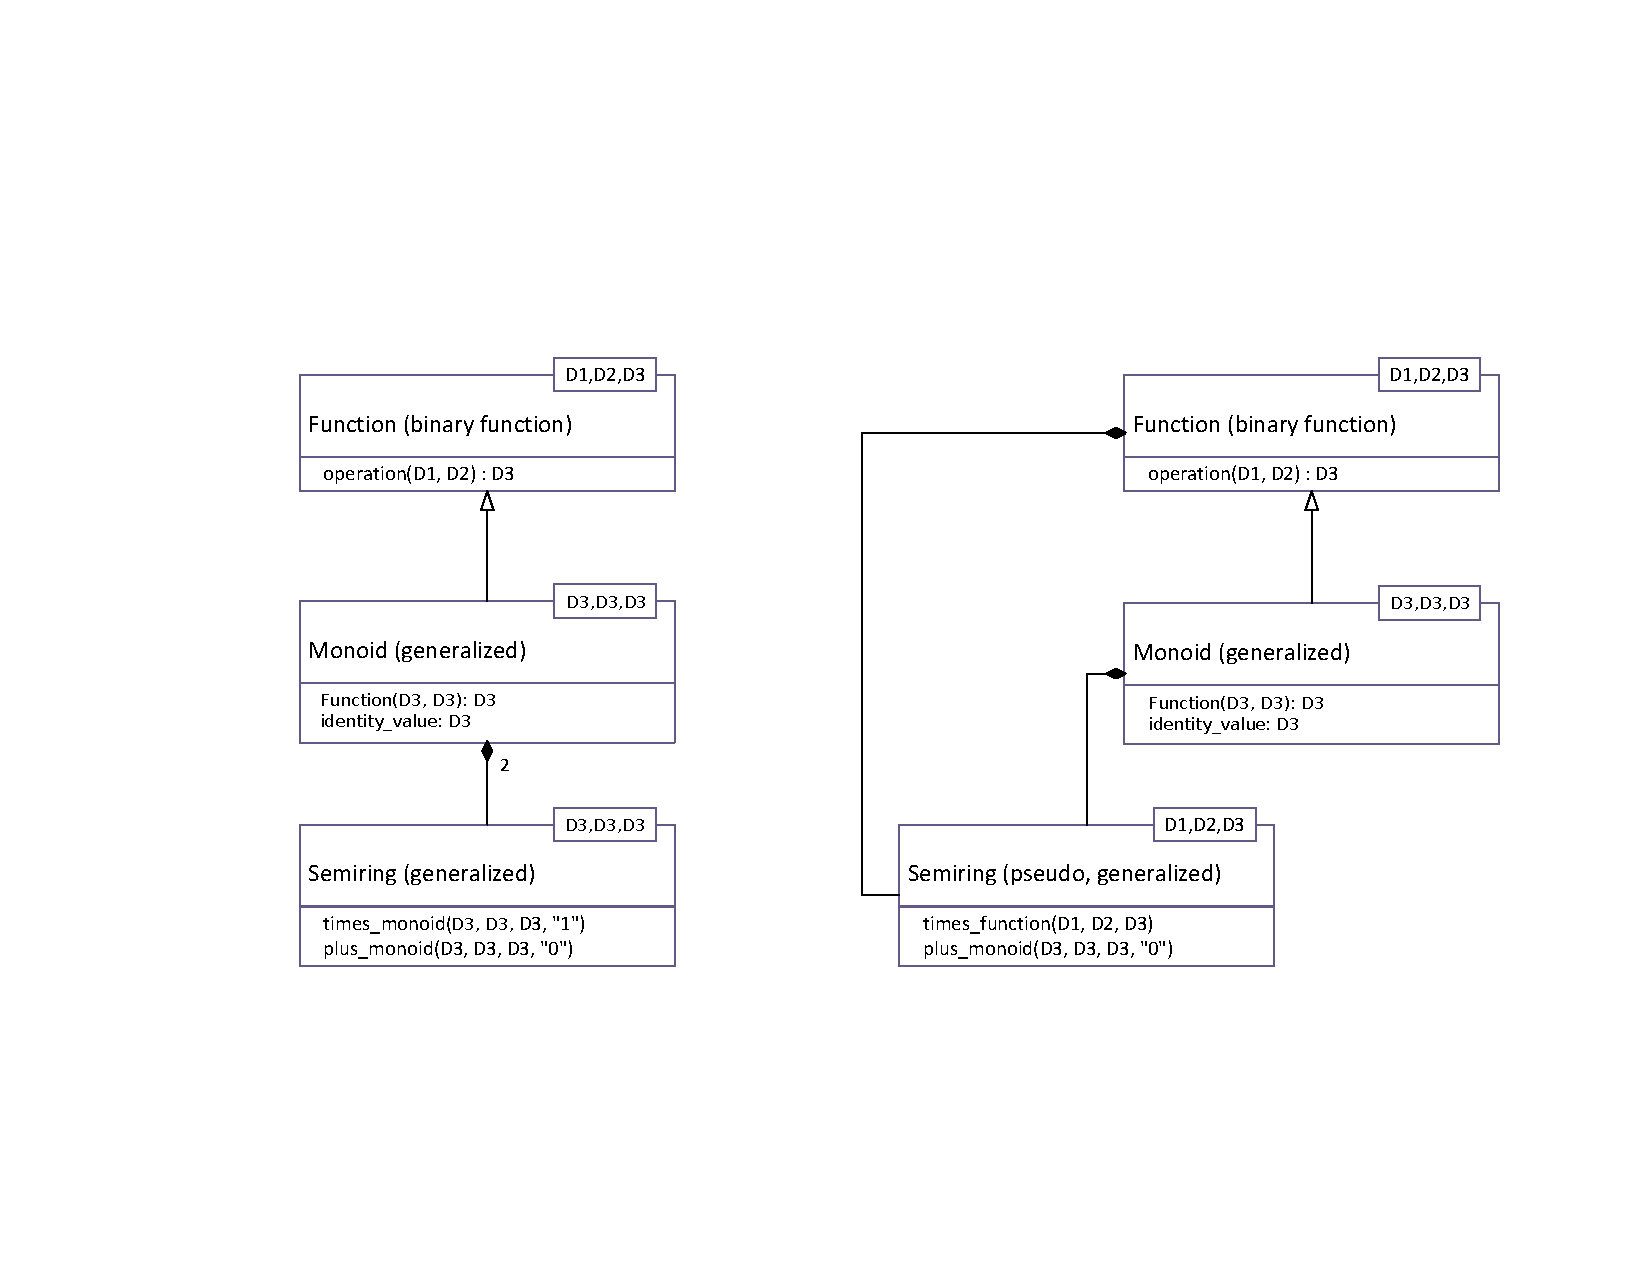
\includegraphics[width=1.0\linewidth,trim=0in 2in 0in 2in]{Algebra_Hierarchy_proposed.pdf}
	\end{center}
	\caption{Hierarchy of object classes in GraphBLAS algebra.}
	\label{Fig:AlgebraHierarchyProposed}
	\hrule
\end{figure}

\begin{table}
	\hrule
	\begin{center}
		\caption{Proposed operator input for relevant GraphBLAS operations. The semiring add and times are shown if applicable.}
		\label{Tab:OperatorInputType}
		\begin{tabular}{l|l|l|l}
			Operation	& Operator Input & Semiring Add & Semiring Times  \\ \hline
			mXm & Semiring & Monoid & Function \\
			&  &  & Monoid \\
			mXv & Semiring & Monoid & Function  \\
			&  &  & Monoid  \\
			ewiseAdd &  Function & n/a & n/a  \\
			& Monoid & n/a & n/a  \\
			ewiseMult & Function & n/a & n/a  \\
			& Monoid & n/a & n/a  \\
			reduce & Monoid & n/a & n/a \\
		\end{tabular}
	\end{center}
	\hrule
\end{table}

\subsection{Vectors}

\scott{Is this strictly sparse vector?} \jose{It is a GraphBLAS vector.}

A vector $\vector{v} = \langle D, N, \{ (i,v_i) \} \rangle$ is defined
by a domain $D$, a size $N>0$ and a set of tuples $(i,v_i)$ where
$0 \leq i < N$ and $v_i \in D$. A particular value of $i$ can only
appear at most once in $\vector{v}$. We define $\bold{n}(\vector{v}) =
N$ and $\bold{L}(\vector{v}) = \{ (i,v_i) \}$. We also define the set
$\vector{i(\vector{v})} = \{ i : (i,v_i) \in \bold{L}(\vector{v}) \}$,
and $\bold{D}(\vector{v}) = D$.

\comment{
\ajy{Overloaded use of $\vector{v}$ in the definition.} \jose{Fixed
through explicitly different fonts.} \scott{OK TO REMOVE}

\ajy{Why not define in terms of $D^{N}$} \jose{It is possible, but seems
more complicated to me.} \scott{OK TO REMOVE}
}

\scott{[snip] If we have a strictly 1D structure,
I believe we must give it an implicit orientation for matrix operations
(I prefer column vector) and discuss all the other vector operations
proposed a while back.}
\jose{I agree that vectors and matrices are more \emph{storage} than
anything else. But I don't think we should add any more properties (\eg,
orientation) than strictly necessary.}

\subsection{Matrices}
\label{Sec:Matrices}

\scott{Is this strictly sparse matrix?}

A matrix $\matrix{A} = \langle D, M, N,  \{ (i,j,A_{ij}) \} \rangle$ is
defined by a domain $D$. its number of rows $M>0$, its number of columns
$N>0$ and a set of tuples $(i,j,A_{ij})$ where $0 \leq i < M$, $0 \leq
j < N$, and $A_{ij} \in D$. A particular pair of values $i,j$ can only
appear at most once in $\matrix{A}$. We define $\bold{n}(\matrix{A})
= N$,  $\bold{m}(\matrix{A}) = M$ and $\bold{L}(\matrix{A}) = \{
(i,j,A_{ij}) \}$.  We also define the sets $\vector{i(\matrix{A})} = \{
i : \exists (i,j,A_{ij}) \in \matrix{A} \}$ and $\vector{j(\matrix{A})}
= \{ j : \exists (i,j,A_{ij}) \in \matrix{A} \}$.  (These are the sets
of nonempty rows and columns of $\matrix{A}$, respectively.)  Finally,
$\bold{D}(\matrix{A}) = D$.

\comment{
\ajy{Overloaded use of $\matrix{A}$ in the definition.}
\jose{Fixed through different fonts.}  \scott{OK TO REMOVE}

\ajy{Why not define in terms of $D^{M \times N}$.}
\jose{It seems more complicated to me.}  \scott{OK TO REMOVE}
}

If $\matrix{A}$ is a matrix and $0 \leq j < N$, then $\matrix{A}(:,j)
= \langle D, M, \{(i,A_{ij}) : (i,j,A_{ij}) \in \bold{L}(\matrix{A})
\} \rangle$ is a vector called the $j$-th \emph{column}
of $\matrix{A}$. Correspondingly, if $\matrix{A}$ is a matrix and
$0 \leq i < M$, then $\matrix{A}(i,:) = \langle D, N, \{(j,A_{ij}) :
(i,j,A_{ij}) \in \bold{L}(\matrix{A}) \} \rangle$ is a vector called
the $i$-th \emph{row} of $\matrix{A}$.

\subsection{Descriptors}

\jose{This was supposed to be just a conceptual introduction to
\emph{Descriptors}. We definitely need more detail. We can add it here
or save for the Section~\ref{Sec:Methods}.}

Descriptors are used as input parameters in various GraphBLAS methods to
provide more details of the operation to be performed by those methods.
In particular, descriptors specify how the other input parameters
should be processed before the main operation of a method is performed.
For example, a descriptor may specify that a particular input matrix
needs to be transposed or that a mask needs to be inverted before using
it in the operation. Some methods may also allow additional processing
of the result before generating the final output parameter.

\scott{'inverted' above is ambiguous, we need to define a better term
like "structural complement".  Further we should specify behaviour if
the mask is a dense container not just when it is sparse.}

For the purpose of constructing descriptors, the parameters of a method
are identified by specific names. The output parameter (typically
the first parameter in a GraphBLAS method) is {\sf OUTP}.  The input
parameters are named {\sf ARG0}, {\sf ARG1}, {\sf ARG2} and so on from
the first input parameter to the last. The mask (typically the next to
last parameter in a method) is named {\sf MASK}. Finally, the descriptor
(typically the last parameter in a method) is not named, since GraphBLAS
does not support modifications of descriptors themselves.

\scott{Is negate/invert/structural complement only restricted to masks?}

\scott{We must specify the behaviour of the descriptor's transpose.
E.g. is it allowed to mutate the operand for the duration of the
operation, or is this strictly a flag that affects the operation only --
how it accesses the operand's values?}


